\documentclass[a4paper, 12pt]{article}

\usepackage[colorlinks=true,urlcolor=blue]{hyperref}
\usepackage[hybrid]{markdown}
\usepackage[a4paper, total={6.5in, 9in}]{geometry}
\usepackage{longtable}
\usepackage{booktabs}

\title{Immobilienrechner Challenge: 2.3 Webservice}
\author{Alexander Shanmugam, Gabriel Torres Gamez, Haris Alic, Si Ben Tran}
\date{16 Januar 2023}

\begin{document}
\maketitle
\newpage

\hypertarget{immoprice-backend}{%
\section{immoprice-backend}\label{immoprice-backend}}

Dieses Backend wurde mit basiert auf Django v4.1.3. Dependencies werden
\href{https://github.com/Immobilienrechner-Challenge/immoprice-backend/blob/main/requirements.txt}{hier}
aufgelistet.

\hypertarget{setup}{%
\subsection{Setup}\label{setup}}

Um die API auf einer Docker Umgebung zu nutzen, muss man die
vorgefertigte Datei
\href{https://github.com/Immobilienrechner-Challenge/immoprice-backend/blob/main/create_docker_container.sh}{create\_docker\_container.sh}
starten und den Container Port 8099 anhand einem nginx Reverse Proxy
freigeben.

\hypertarget{setup-ohne-reverse-proxy}{%
\paragraph{Setup ohne Reverse Proxy}\label{setup-ohne-reverse-proxy}}

Falls man die API nicht hinter ein nginx Reverse Proxy laufen lassen
will, müsste man die Netzwerkeinstellungen in der
\href{https://github.com/Immobilienrechner-Challenge/immoprice-backend/blob/main/create_docker_container.sh}{create\_docker\_container.sh}
Datei anpassen:

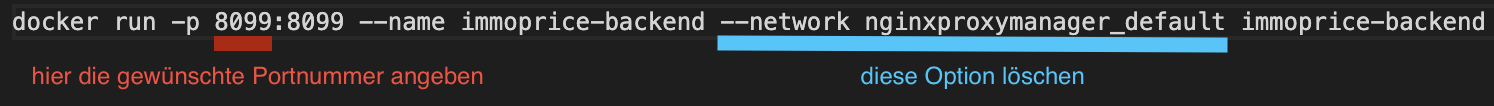
\includegraphics[width=\linewidth]{img/EinstellungDocker.png}

\newpage
\hypertarget{hosting}{%
\subsection{Hosting}\label{hosting}}

Das Hosting des Backends findet auf einer Docker Umgebung statt. Alle
anfragen werden durch den Reverse Proxy auf
\href{https://api.immoprice.ch}{https://api.immoprice.ch} auf das
Backend weitergeleitet.


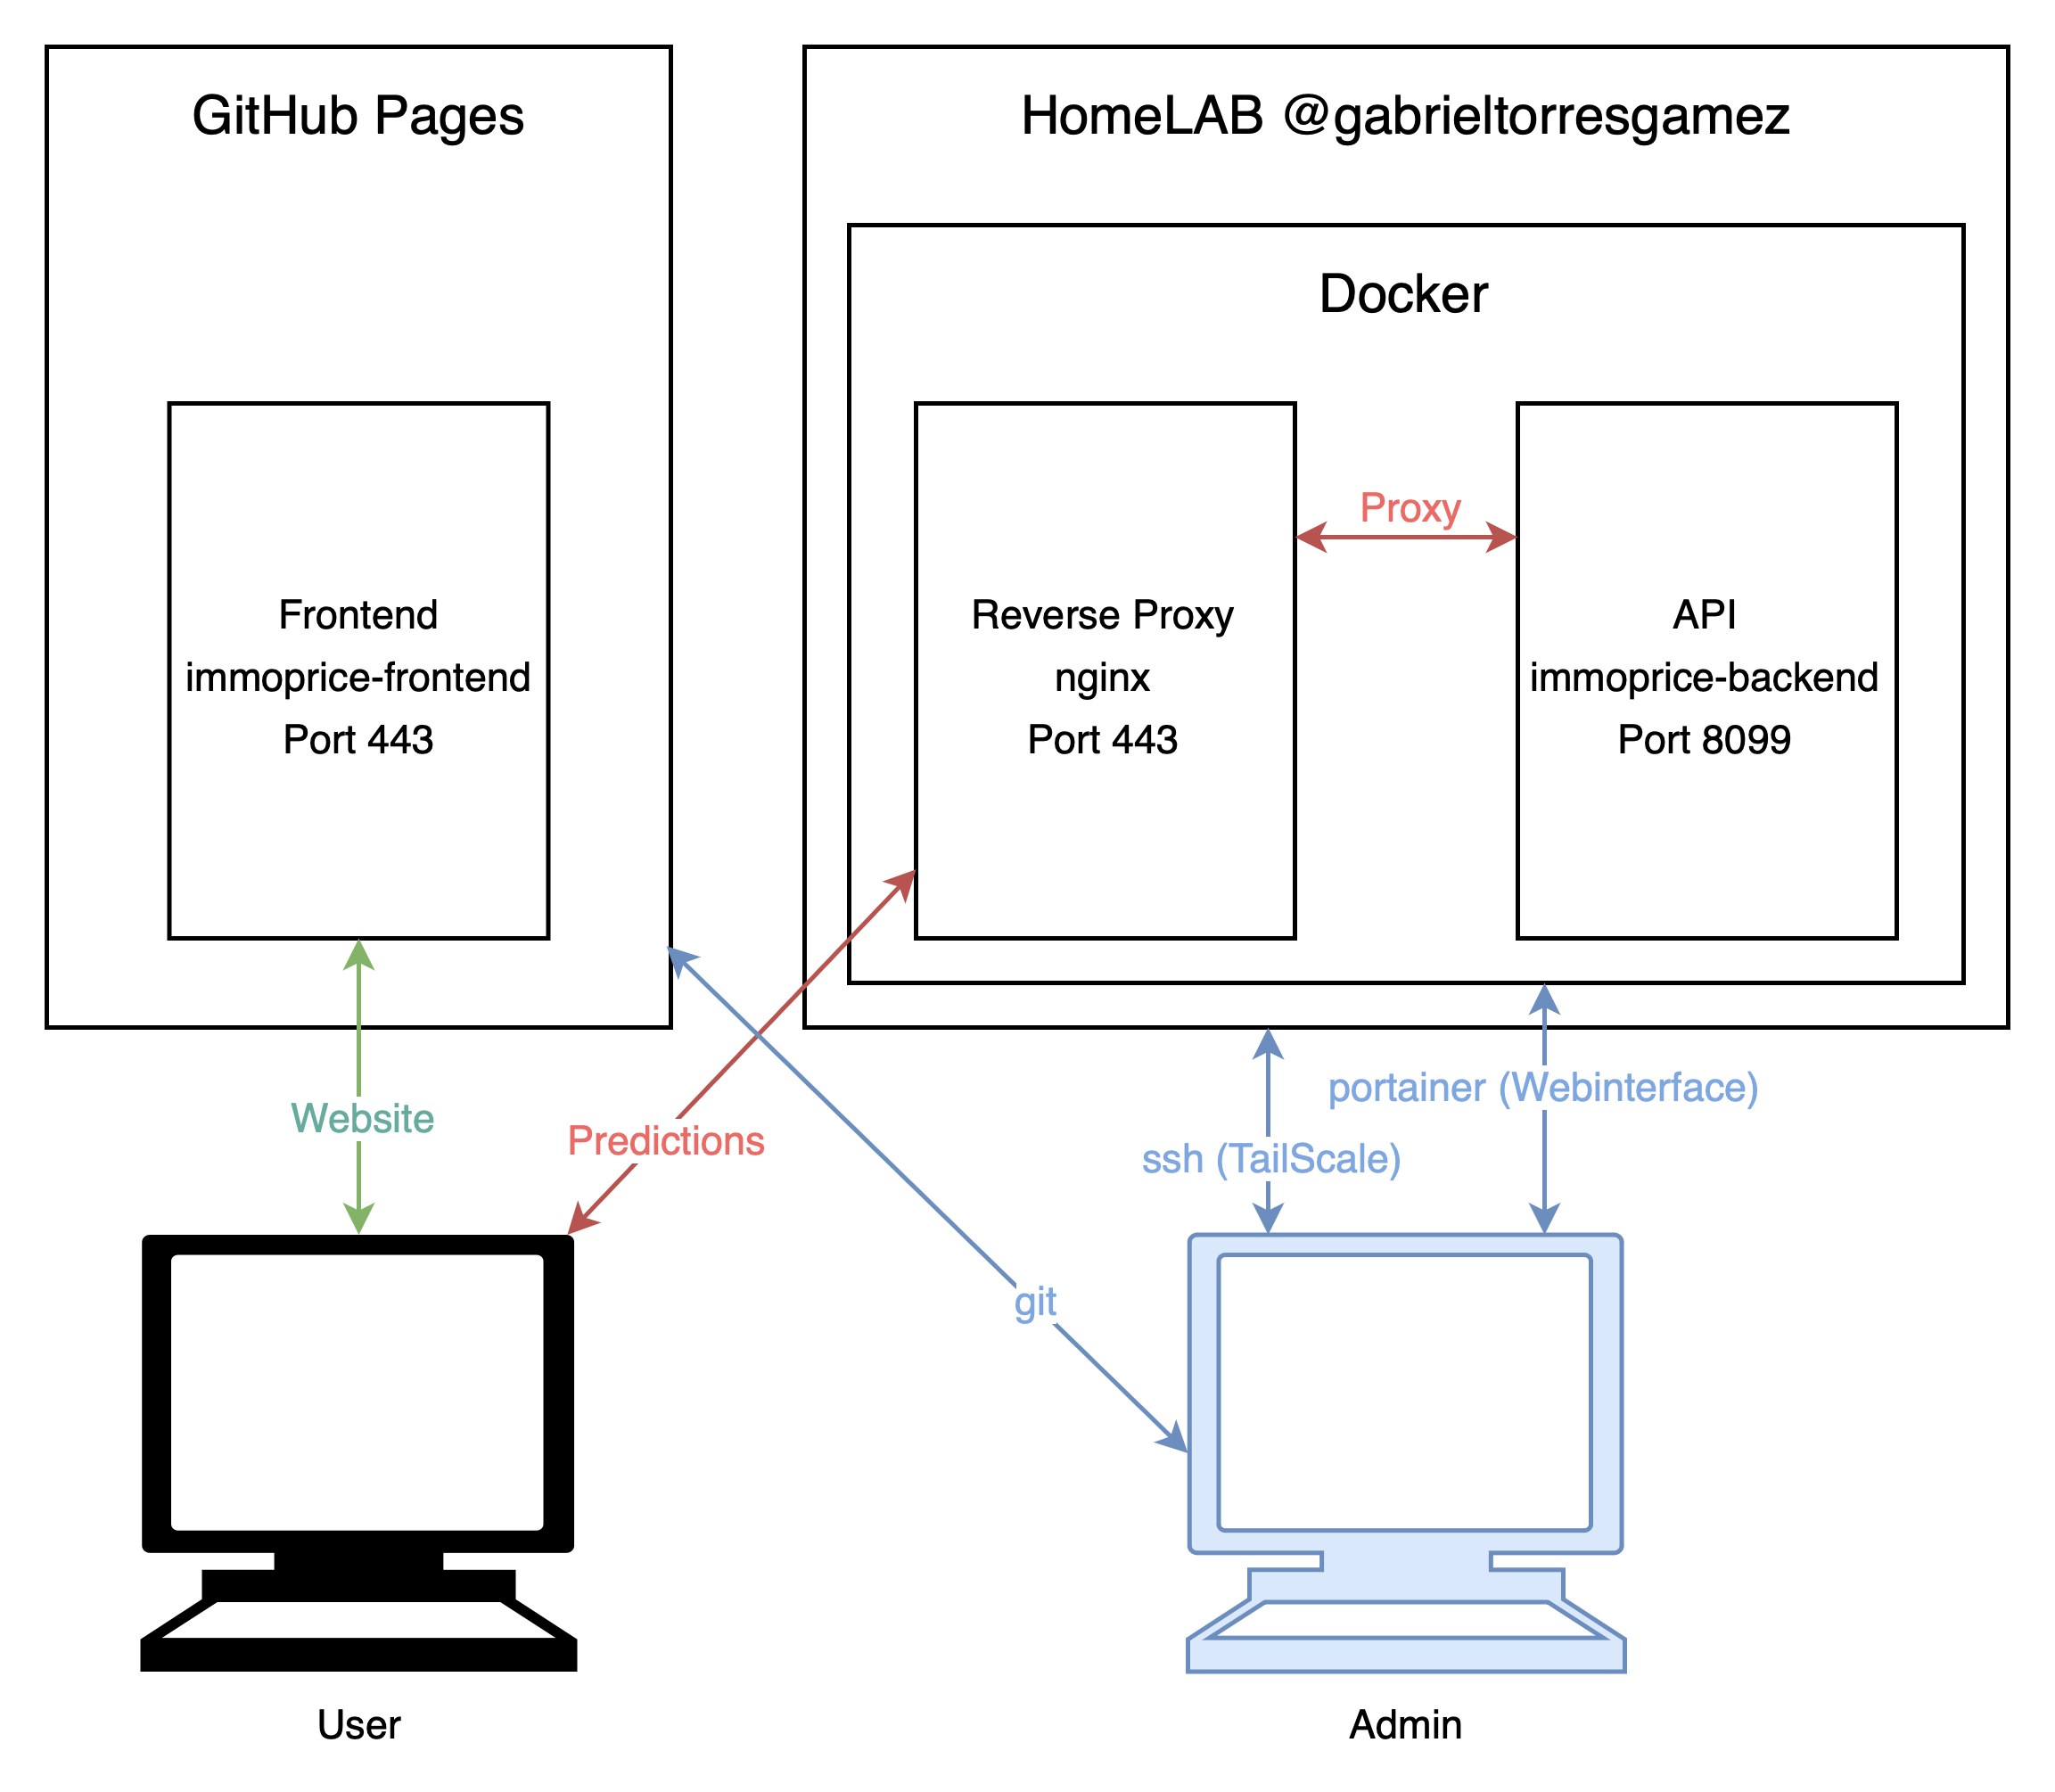
\includegraphics[width=\linewidth]{img/SetupDocker.png}

\newpage
\hypertarget{schnittstellen}{%
\subsection{Schnittstellen}\label{schnittstellen}}

Hier wird die relevante Schnittstelle erfasst:

\begin{longtable}[]{@{}ll@{}}
\toprule
model1 &\tabularnewline
\midrule
\endhead
URL & \href{https://api.immoprice.ch/model1/}{model1/}\tabularnewline
Request Type & GET\tabularnewline
Beschreibung & Modell zur Vorhersage von Immobilienpreisen auf
\href{https://immoprice.ch}{immoprice.ch}\tabularnewline
Input 1 & living\_space(float)\tabularnewline
Input 2 & type(string)\tabularnewline
Input 3 & rooms(float)\tabularnewline
Input 4 & zip\_code(int)\tabularnewline
Input 5 & floor\_space(float)\tabularnewline
Input 6 & plot\_area(float)\tabularnewline
Input 7 & last\_refurbishment(int)\tabularnewline
Input 8 & year\_built(int)\tabularnewline
Output & price(float)\tabularnewline
Beispiel &
\href{https://api.immoprice.ch/model1/?living_space=200\&type=villa\&rooms=10\&zip_code=8050\&floor_space=300\&plot_area=500\&last_refurbishment=2020\&year_built=2010}{Hier}\tabularnewline
\bottomrule
\end{longtable}

\hypertarget{bekannte-probleme}{%
\paragraph{Bekannte Probleme}\label{bekannte-probleme}}

Das Modell wurde nur auf eine kleine Stichprobe der Daten in der Schweiz
trainiert. Deswegen können einige Prognosen eine starke Abweichung vom
realen Preis haben. Das Modell ist nicht in der Lage spezielle Fälle,
wie z.B. wertvolle Aussichten, Immobilienlage an einem speziellen Ort,
Innenausstattung oder historische Signifikanz miteinberechnen.

\hypertarget{cross-origin-restrictions}{%
\subsection{Cross-Origin
Restrictions}\label{cross-origin-restrictions}}

Es können Cross-Origin Restriction Fehler auftauchen, da die API
konfiguriert ist, Anfragen aus
\href{https://immoprice.ch}{https://immoprice.ch} zu verarbeiten. Falls
dies auftritt, muss die Option im Browser manuell deaktiviert werden.

\hypertarget{immoprice-frontend}{%
\section{immoprice-frontend}\label{immoprice-frontend}}

In diesem Repository wird unsere Seite
\href{https://immoprice.ch}{immoprice.ch} entwickelt, versioniert und
verwaltet. Die neuste Version des main Branches wird anhand von GitHub
Pages unter der oben genannten URL zur Verfügung gestellt. Die
Funktionalität der Webseite wurde anhand
\href{https://jquery.com}{jQuery} umgesetzt. Keine Installation wird zur
Weiterentwicklung benötigt.

\hypertarget{api}{%
\subsection{API}\label{api}}

Um eine Preisvorhersage zu generieren, machen wir AJAX Abfragen an unser
Backend
\href{https://github.com/Immobilienrechner-Challenge/immoprice-backend}{immoprice-backend}.
Weiter Informationen sind unter der
\href{https://github.com/Immobilienrechner-Challenge/docs/blob/main/Repositories/immoprice-backend/Dokumentation.md}{Dokumentationsseite
des Backend} verfügbar.

\end{document}
